\documentclass{standalone}
\usepackage{tikz}
\usepackage{ctex,siunitx}
\setCJKmainfont{Noto Serif CJK SC}
\usepackage{tkz-euclide}
\usepackage{amsmath}
\usetikzlibrary{patterns, calc,3d}
\usetikzlibrary {decorations.pathmorphing,decorations.pathreplacing,decorations.shapes}
\tikzset{label style/.append style={font=\small}}
\begin{document}
\small
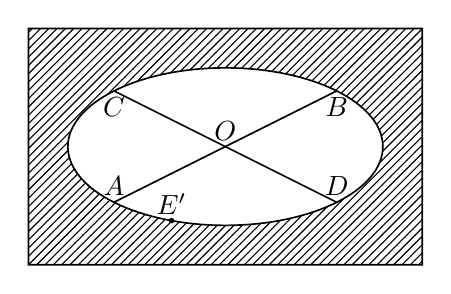
\begin{tikzpicture}[>=latex,scale=1.0,inner sep=2pt]
  \draw[semithick,even odd rule,pattern=north east lines](-2.5,-1.5)rectangle(2.5,1.5)(0,0)ellipse(2 and 1);
  \draw[semithick]({2*cos(45)},{sin(45)})node[below]{$B$}--({2*cos(225)},{sin(225)})node[above]{$A$};
  \draw[semithick]({2*cos(135)},{sin(135)})node[below]{$C$}--({2*cos(-45)},{sin(-45)})node[above]{$D$};
  \node at (0,0)[above]{$O$};
  \fill ({2*cos(250)},{sin(250)})circle(1pt)node[above]{$E'$};
\end{tikzpicture}
\end{document}